\section{Overview}
\label{sec:buffer-control}
RxJava points out on its wiki page \cite{RxJava-Wiki-Backpressure} about backpressure that it does not make the problem of overproduction in the source go away. It claims to only move ``\textit{the problem up the chain of operators to a point where it can be handled better}''. To do so, they created the \textit{reactive pull} mechanism with operators like \code{onBackpressureBuffer} and \code{onBackpressureDrop}, such that the flow control is moved up to these kinds of operators.

We propose to move this flow control even further up the chain; up to the point where the source of the stream is drained in the pipeline of operators. Only there we can have maximum control over how much data is brought into the stream at a particular point in time. With this we do not have the need for infinite buffers as is the case in \code{onBackpressureBuffer}, nor do we have to drop unprocessed elements as is done with \code{onBackpressureDrop}. We propose to not wrap the cold source in the \code{Observable.create} (or any of its derived factory methods) but to wrap it in a universal, interactive interface. This way we are not dependent in our implementation on what kind of source we are dealing with. Given this interactive interface we can fill a \textit{bounded} buffer with as many elements as can be processed at a particular point in time. The buffer pulls data from the source on behalf of the subscriber, which gets as much data pushed at it as it is able to handle. Pushing an element from the buffer to the downstream will automatically block the thread for another element to be pushed until the first one is fully processed.

To control the buffer's size, we will use feedback control. This makes total sense, as we don't know how fast the downstream is going to drain the buffer. However, it does not make any sense to give a certain size to the setpoint and compare the current size with it, as some `slow' consumers might go faster or slower than expected. Bounding the buffer to a certain fixed size defeats the purpose of the feedback system in this case, as we cannot dynamically grow or shrink the size as needed. On the other hand, it is also not possible to ask ``\textit{make sure the buffer is filled to its optimal size}''. A feedback system is not able to solve this, as it does not have a particular setpoint specified.

Instead of controlling the buffer size directly, we choose to measure the ratio between what goes out the buffer and what comes in the buffer. We will refer to this ratio as the system's throughput. In an optimal situation the amount of data that comes in is just as much as comes out of the system, so ideally this ratio must be $1.0$, which will be the setpoint of this system. Given the error that comes from the difference between the setpoint and the actual throughput, we can then determine how many elements to request from the source in the next iteration. The controller that does this will be discussed in a later section.

The full feedback system is depicted in \Cref{fig:backpressure-feedback-system}. Here it is also clearly visible that the source itself is \emph{not} part of the feedback system, but is \emph{used} by the system to retrieve a certain number of elements from. Also note that the \textit{downstream handler} is not part of feedback system. Even though it \emph{interacts} with the buffer, it is an external force that influences the behavior of the system. Ultimately the \textit{downstream handler} is the part that exposes an \obs for an \obv to listen to.

\begin{figure}[H]
	\begin{center}
		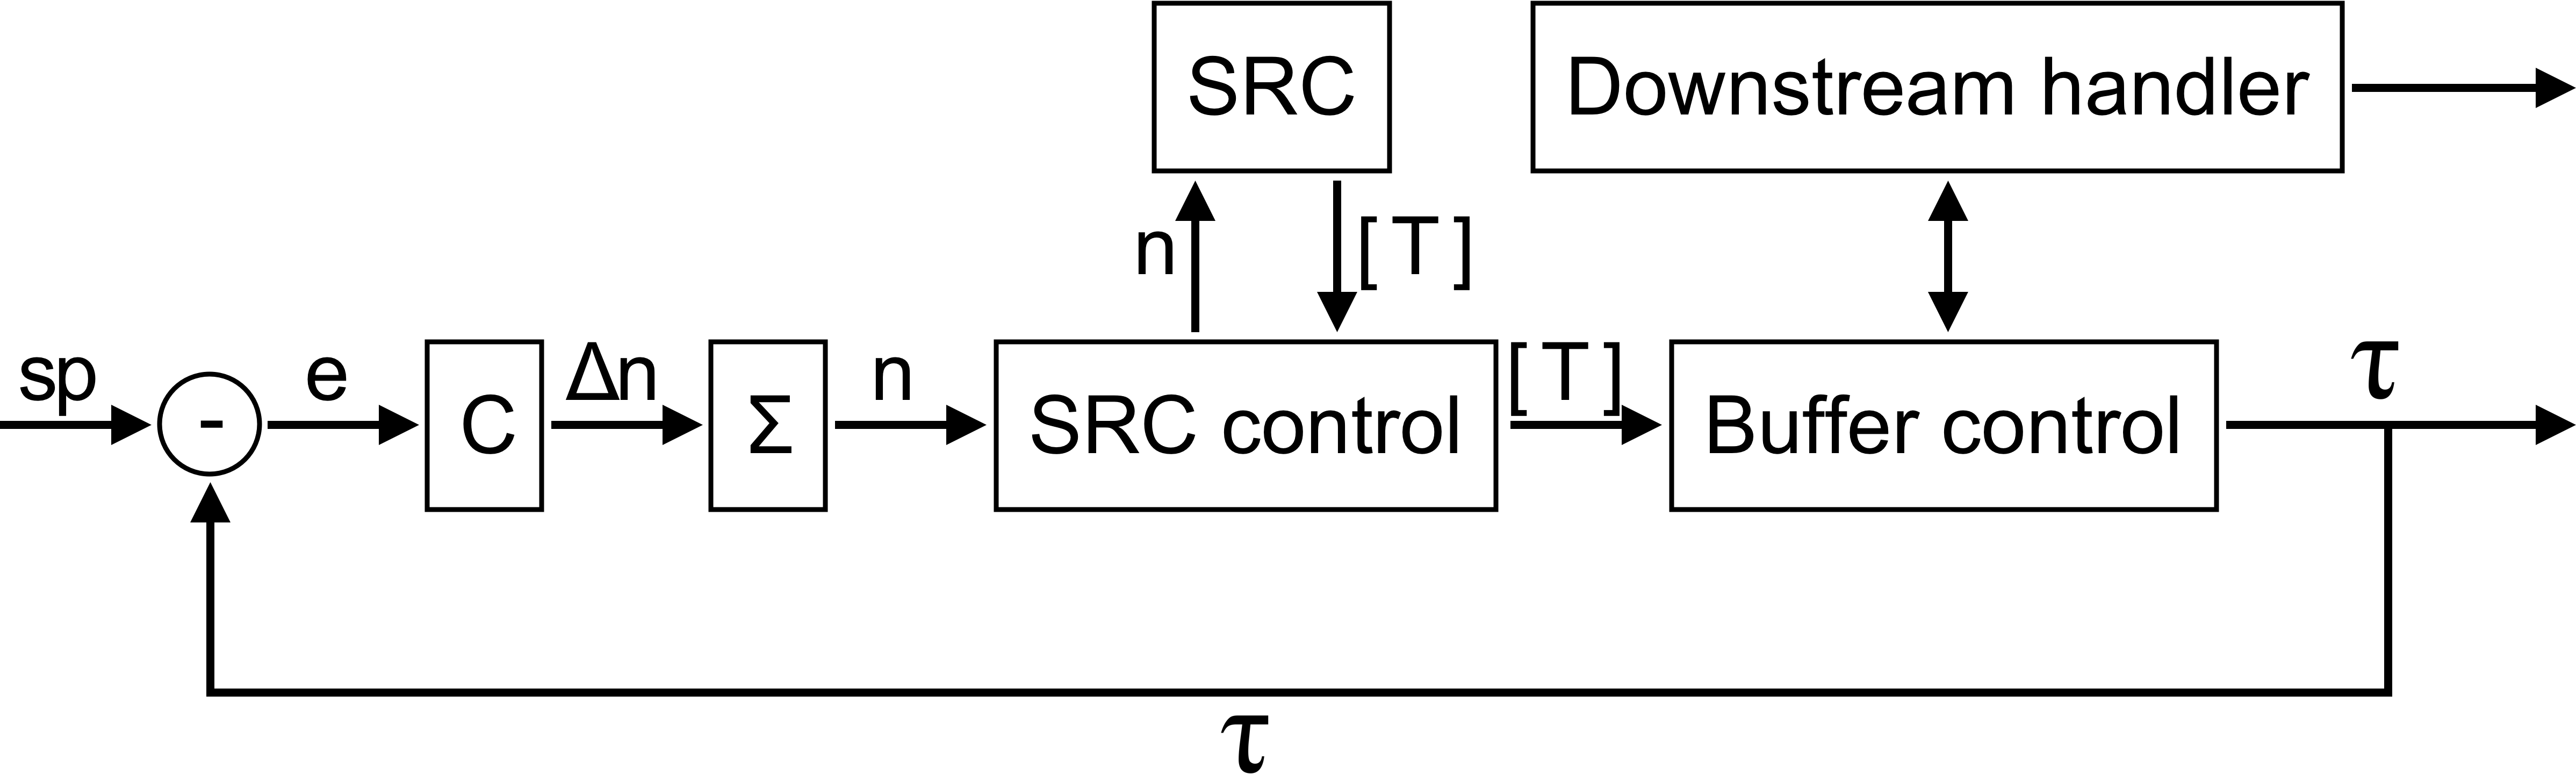
\includegraphics[width=0.8\textwidth]{figures/Backpressure-feedback-system.png}
	\end{center}
	\caption{Feedback system for controlling overproduction}
	\label{fig:backpressure-feedback-system}
\end{figure}

In the rest of this section we will go into the details of this feedback system and discuss both the theoretical background and implementations.
